%!TeX root=main.tex
\chapter{پرسش و پاسخ تصویری}
\thispagestyle{empty}

مجموعه داده
\href{https://visualqa.org/vqa_v1_download.html}{\lr{Visual Question Answering (VQA v1.0)}}
یکی از غنی‌ترین و معروف‌‌ترین مجموعه داده در مسئله پرسش و پاسخ تصویری می‌باشد. یک تصویر و یک سوال مرتبط با تصویر به عنوان ورودی به سیستم داده می‌شود. هدف این است که با توجه به تصویر، دقیق‌ترین پاسخ به سوال داده شود. این مجموعه داده شامل 250 هزار تصویر و 760 هزار سوال و 10 میلیون پاسخ می‌باشد. تصاویر این مجموعه داده از دو بخش تصاویر حقیقی
\LTRfootnote{\lr{Real Image}}
و تصاویر انتزاعی
\LTRfootnote{\lr{Abstract Image}}
تشکیل شده است  \cite{antol2015vqa}.
\section{تصاویر حقیقی مجموعه داده
	\lr{VQA}}
برای تصاویر حقیقی (که شامل 123289 داده آمورشی و 81434 داده ارزیابی می‌باشد) از تصاویر موجود در مجموعه داده  
\lr{ MS COCO} \LTRfootnote{\lr{Microsoft Common Objects In Context (MS COCO)}} \cite{lin2015microsoft}
استفاده شده است. هر تصویر مجموعه داده 
\lr{MS COCO}
شامل چندین شی است. درجه سختی تصاویر، این مجموعه داده را مناسب برای تسک  
\lr{VQA}
کرده است. در شکل \ref{vqa-v1real} نمونه‌ای از تصاویر حقیقی به همراه پرسش و پاسخ مربوطه آورده شده است.

\begin{figure}
	\center{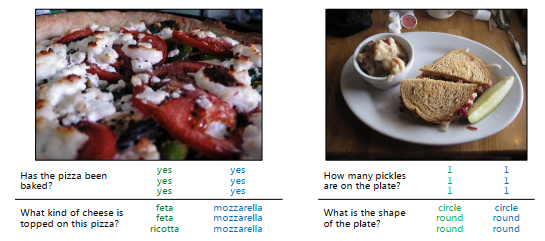
\includegraphics{images/VQA_V1-real-image.PNG}}
	\caption{چند نمونه از تصاویر حقیقی مجموعه داده  \lr{VQA v1}
	به همراه سوالات و زیر مجموعه‌ای از پاسخ‌ها. پاسخ‌های سبز رنگ با نگاه به تصویر داده شده است. پاسخ آبی بدون نگاه به تصویر داده شده است.  \cite{antol2015vqa}}
	\label{vqa-v1real}
\end{figure}

\section{تصاویر انتزاعی مجموعه داده
	\lr{VQA}}
تصاویر انتزاعی شامل تصاویر کارتونی می‌باشد. علت قرار دادن تصاویر انتزاعی در کنار تصاویر حقیقی این است که با از بین بردن نیاز به تجزیه و تحلیل تصویر واقعی، تمرکز مدل بر روی استدلال‌های سطح بالاتر افزایش یابد. تصاویر انتزاعی شامل هر دو محیط داخل خانه و خارج خانه می‌باشند. این مجموعه شامل 100 شی و 31 حیوان در موقعیت‌های مختلف می‌باشد. 50 هزار داده از تصاویر انتزاعی در مجموعه 
\lr{VQA}
موجود است. در شکل \ref{vqa-v1abs} نمونه‌ای از تصاویر انتزاعی به همراه پرسش و پاسخ مربوطه آورده شده است.

\begin{figure}[H]
	\center{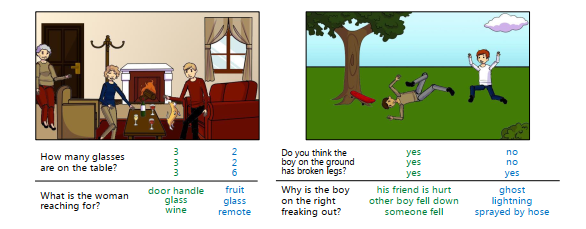
\includegraphics{images/VQA_V1-abs-image.PNG}}
	\caption{چند نمونه از تصاویر انتزاعی مجموعه داده \lr{VQA v1} \cite{antol2015vqa}}
	\label{vqa-v1abs}
\end{figure}

\section{نوع سوالات و نحوه جمع‌آوری مجموعه داده
	\lr{VQA}}
به ازای هر تصویر در مجموعه داده
\lr{VQA}
حداقل 3 سوال (به طور میانگین 4 یا 5 سوال) وجود دارد که 10 کاربر مختلف به هر سوال پاسخ داده‌اند. پرسش‌های بله/خیر، تعداد اشیا و دیگرپرسش‌ها دسته‌بندی انواع سوالات در این مجموعه داده می‌باشد. برای پاسخ‌گویی به سوالات از کاربران حقیقی استفاده شده است و کاربر می‌بایست از بین گزینه‌های موجود پاسخ مناسب سوال را انتخاب کند (شکل\ref{vqa-ui}).

\begin{figure}[H]
	\center{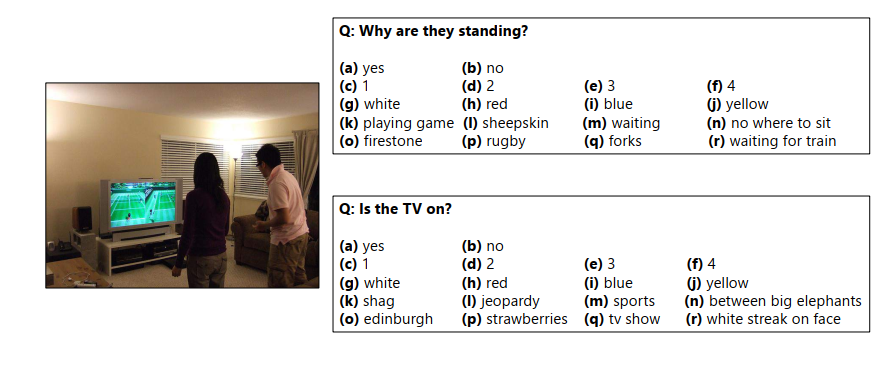
\includegraphics[width=0.9\linewidth]{images/VQA-V1-ui.PNG}}
	\caption{نمونه‌ای  سوالات چند  گزینه‌ای برای یک تصویر در  
	\lr{VQA v1} \cite{antol2015vqa}}
	\label{vqa-ui}
\end{figure}

\section{مجموعه داده
	\lr{VQA v2.0}}
مجموعه داده
\lr{VQA v2.0} 
در سال 2017 در تکمیل و بهبود مجموعه داده 
\lr{VQA v1.0} 
معرفی شد. مشکل اصلی مجموعه داده 
\lr{VQA v1.0}
تعصبات زبانی
\LTRfootnote{\lr{language-bias}}
موجود می‌باشد. به عنوان مثال اگر سوال با 
\lr{Is there a clock}
آغاز شود، با احتمال 95 درصد پاسخ
\lr{yes}
می‌باشد. غلبه بر این مشکل با جمع‌آوری تصاویر مکمل میسر شد. به این صورت که به ازای هر پرسش یکسان دو تصویر وجود دارد که پاسخ‌های متفاوتی دارند. در شکل \ref{VQA_V2} نمونه‌ای از مجموعه داده
\lr{VQA v1.0} 
قابل مشاهده است \cite{balanced_vqa_v2}.

\begin{figure}[H]
	\center{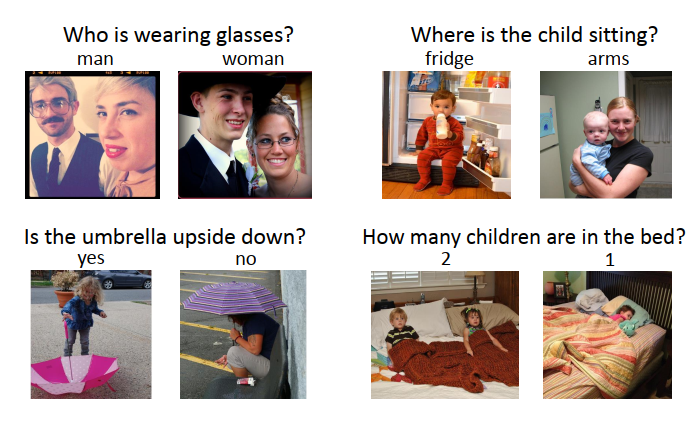
\includegraphics[width=0.9\linewidth]{images/VQA_V2.PNG}}
	\caption{چند نمونه از مجموعه داده  
	\lr{VQA v2.0} \cite{balanced_vqa_v2}}
	\label{VQA_V2}
\end{figure}

با جمع‌آوری مجموعه داده
\lr{VQA v2.0} 
به عنوان نسخه متعادل شده مجموعه داده معروف
\lr{VQA v1.0}، تعصبات زبانی به میزان قابل توجهی کاهش پیدا کرد. همچنین وجود تصاویر مکمل باعث شد دقت به دست‌آمده در مدل‌های زبانی-بصری  قابل اطمینان‌تر باشد و فهم مدل از تصویر را انعکاس دهد.

